    \documentclass{article}
    \usepackage{paquetes/caratula}
    \usepackage[a4paper, left=2.5cm, right=2.5cm, bottom=2.5cm, top=3.0cm]{geometry}
    \usepackage{indentfirst}
    \usepackage{graphicx}
    \usepackage{subcaption}
    \usepackage{amsmath}
    \usepackage{amssymb}
    \usepackage{xcolor}
    \usepackage{float}
    \usepackage{graphicx}
    \usepackage{makecell}



    \makeindex

    \renewcommand\theadalign{bc}
\renewcommand\theadfont{\bfseries}
\renewcommand\theadgape{\Gape[4pt]}
\renewcommand\cellgape{\Gape[4pt]}

    \begin{document}

    \titulo{Trabajo Práctico 1}
    \subtitulo{Programación Lineal}
    \fecha{1$^{\text{er}}$ cuatrimestre 2025}
    \materia{Investigación Operativa}

    \integrante{Guibaudo, Camila}{682/17}{camiguiba@gmail.com}
    \integrante{Azar, Agustin}{693/21}{Agustin.azar101@gmail.com}
    \integrante{Pages, Julieta}{1691/21}{julib.pages@gmail.com}

    \maketitle

    \newpage

    %%%%%%%%%%%%%%%%%%%%%%%%%%%%%%%%%%%%%%%%%%%%%%%%%%%%%%%%%%%%%%%%%%%%%%%%%%%%%%%%%%%%%%%%%%%%
    %%%%%%%%%%%%%%%%%%%%%%%%%%%%%%         Modelos de PE      %%%%%%%%%%%%%%%%%%%%%%%%%%%%%%%%%%
    %%%%%%%%%%%%%%%%%%%%%%%%%%%%%%%%%%%%%%%%%%%%%%%%%%%%%%%%%%%%%%%%%%%%%%%%%%%%%%%%%%%%%%%%%%%%
    \section{Modelos}
    Se nos presentó un problema donde una empresa debe distribuir productos a varios clientes, y quiere incorporar una nueva metodología para hacerlo. Entonces, para ver si podría ser conveniente, se desarrollaron tres modelos. El primero para representar el Modelo Actual de distribución donde solo se cuenta con un camión para hacer todos los repartos. Este modelo coincide con el modelo del \textit{The Traveling Salesman Problem (Modelo Actual)}. Luego se realizó un modelo que pasa a incluir la opción de realizar ciertas entregas en bici o a pie desde un punto por el que pasara el camión, sujeto a ciertas restricciones. Y por último, vamos a tener un tercer modelo que consiste en agregar al modelo anterior un par de restricciones que serían deseables, y nos interesa ver cuánto se perdería en caso de tenerlas en cuenta. \\
    En adelante, llamaremos Modelo Actual al modelo que maneja actualmente la empresa, donde solo se cuenta con un camión, Nuevo Modelo al modelo que permite el uso de repartidores, y Modelo Adicional a su versión con restricciones deseables.

    %%%%%%%%%%%%%%%%%%%%%%%%%%%%%%         Modelo Actual      %%%%%%%%%%%%%%%%%%%%%%%%%%%%%%%%%%
    \subsection{Modelo Actual (Modelo Actual):} \label{modelo_actual}
    \subsection*{Variables}
    \begin{align*}
        x_{i\_j} &\in \{0,1\} && \text{1 si se viaja del nodo } i \text{ al nodo } j \\
        u_i &\in \mathbb{R} && \text{Variable auxiliar para eliminación de subciclos (MTZ)}
    \end{align*}

    \subsection*{Restricciones}

    \paragraph{1. Visitar una única vez cada cliente}
    \[
    \sum_{j=1}^{n} x_{i\_j} = 1 \quad \forall i \in \{1, \dots, n\}
    \]

    \paragraph{2. Conservación de flujo}
    \[
    \sum_{\substack{j=1 \\ j \ne i}}^{n} x_{i\_j} - \sum_{\substack{j=1 \\ j \ne i}}^{n} x_{j\_i} = 0 \quad \forall i \in \{1, \dots, n\}
    \]

    \paragraph{3. Eliminación de subciclos / detour (MTZ)}
    \[
    u_i - u_j + (n - 1)x_{i\_j} \leq n - 2 \quad \forall i, j \in \{2, \dots, n\},\ i \ne j
    \]

    \[
    u_1 = 0
    \]

    \[
    1 \leq u_i \leq n - 1 \quad \forall i \in \{2, \dots, n\}
    \]

    %%%%%%%%%%%%%%%%%%%%%%%%%%%%%%         Nuevo Modelo      %%%%%%%%%%%%%%%%%%%%%%%%%%%%%%%%%%
    \subsection{Nuevo Modelo:} \label{model_repartidores}
    \subsection*{Variables}
    \begin{align*}
        x_{i\_j} &\in \{0,1\} && \text{1 si se va del nodo } i \text{ al nodo } j \text{ en camión }\\
        u_i &\in \mathbb{R} && \text{Variable auxiliar para eliminación de subciclos (MTZ)} \\
        r_{i\_j} &\in \{0,1\} && \text{1 si se va del nodo } i \text{ al nodo } j \text{ con repartidor (bici) } \\
        d_{i} &\in \{0,1\} && \text{1 si el nodo $i$ es depósito }
    \end{align*}

    \subsection*{Parámetros}
    \begin{itemize}
        \item \( n \): Número total de nodos (clientes + depósito)
        \item \( i, j \in \{1, \dots, n\} \)
        \item El nodo \(1\) representa el depósito
    \end{itemize}

    \subsection*{Restricciones}

    \paragraph{1. Solo un depósito activo}
    \[
    \sum_{i=1}^{n} d_i = 1
    \]

    \paragraph{2. El camión pasa máximo una vez por cliente}
    \[
    \sum_{i=1}^{n} x_{i\_j} \leq 1 \quad \forall j \in \{1, \dots, n\}
    \]

    \paragraph{3. Conservación de flujo (camión)}
    \[
    \sum_{\substack{j=1 \\ j \ne i}}^{n} x_{i\_j} - \sum_{\substack{j=1 \\ j \ne i}}^{n} x_{j\_i} = 0 \quad \forall i \in \{1, \dots, n\}
    \]

    \paragraph{4. El repartidor solo sale de nodos por los que pasó el camión}
    \[
    \sum_{k=1}^{n} x_{k\_i} + d_i - r_{i\_j} \geq 0 \quad \forall i,j \in \{1, \dots, n\}
    \]

    \paragraph{5. Cumplir la distancia máxima para el repartidor}
    \[
    r_{i\_j} \cdot \text{dist}_{i\_j} \leq d_{\text{max}} \quad \forall i,j \in \{1, \dots, n\}
    \]

    \paragraph{6. Eliminación de subciclos / detour (MTZ)}
    \[
    u_i - u_j + (n - 1) x_{i\_j} - n d_i - n d_j \leq n - 2 \quad \forall i \ne j,\ i,j \in \{1, \dots, n\}
    \]
    \begin{align*}
    u_i + d_i &\geq 1 \quad \forall i \in \{1, \dots, n\} \\
    u_i + n \cdot d_i &\leq n \quad \forall i \in \{1, \dots, n\}
    \end{align*}
    (si $i$ es el depósito ($d_i=1$) entonces no le pedimos nada)

    \paragraph{7. Asegurar la visita a cada cliente}
    \[
    \sum_{k=1}^{n} (x_{k\_j} + r_{kj}) + d_j \geq 1 \quad \forall j \in \{1, \dots, n\}
    \]
    O llego con camión, o llego con repartidor, o soy el depósito.

    \paragraph{8. Máximo una entrega refrigerada por nodo}
    \[
    \sum_{j \in R} r_{i\_j} \leq 1 \quad \forall i \in \{1, \dots, n\}
    \]
    donde \( R \subseteq \{1, \dots, n\} \) es el conjunto de clientes con productos refrigerados.




    \subsection{Modelo Adicional con clientes requeridos:} \label{modelo1}

    Este modelo es una extensión del nuevo modelo donde se incorpora la restricción desdeada por la empresa de que determinados clietnes deben ser atendidos exclusivamente por el camión.

    La función objetivo, las variables y las restricciones son iguales a las del modelo anterior. Solo se agregan la siguiente restricción:
    \subsubsection*{Restricciones adicionales}

    \paragraph{Clientes exclusivos para camión} . \\
    Si un nodo $i$ es un cliente exclusivo, entonces un camión debe pasar por él
    \[
    \sum_{j=1}^{n} x_{i\_j} + d_{i} \geq 1 \quad \forall i \in E
    \]
    donde $E$ es el conjunto de clientes exclusivos.

    \subsection{Modelo Adicional de repartidores:} \label{modelo1}

    En este modelo agregamos la restricción de que cada repartidor que se utilice debe realizar al menos 4 entregas.

    La función objetivo, las variables y las restricciones son iguales a las del modelo anterior. Solo se agregan las siguientes variables y restricciones adicionales:

    \subsubsection*{Variables adicionales}

    \begin{align*}
        r_{i} &\in \{0,1\} && \text{1 si al menos un repartidor parte del nodo } i
    \end{align*}

    \subsubsection*{Restricciones adicionales}

    \paragraph{1. Restricciones para mínimo 4 entregas por repartidor}.  \\

    Si un repartidor parte del nodo $i$, entonces debe realizar al menos cuatro entregas.
    \[
    \sum_{j=1}^{n} r_{i\_j} - 4 \cdot r_{i} \geq 0 \quad \forall i \in \{1, \dots, n\}
    \]

    Si un repartidor parte del nodo $i$, entonces $r_i = 1$
    \[
    \sum_{j=1}^{n} r_{i\_j} - n \cdot r_{i} \leq 0 \quad \forall i \in \{1, \dots, n\}
    \]


    \subsection{Modelo Adicional con restricciones combinadas:} \label{modelo1}
    En adicción a los modelos adicionales previamente explicados agregamos un nuevo modelo en el cual combinamos ambas restricciones adicionales propuestas por el cliente.
    \subsubsection*{Variables adicionales}

    \begin{align*}
        r_{i} &\in \{0,1\} && \text{1 si al menos un repartidor parte del nodo } i
    \end{align*}

    \subsubsection*{Restricciones adicionales}

     \paragraph{Clientes exclusivos para camión} . \\
    Si un nodo $i$ es un cliente exclusivo, entonces un camión debe pasar por él
    \[
    \sum_{j=1}^{n} x_{i\_j} + d_{i} \geq 1 \quad \forall i \in E
    \]
    donde $E$ es el conjunto de clientes exclusivos.
    \paragraph{1. Restricciones para mínimo 4 entregas por repartidor}.  \\

    Si un repartidor parte del nodo $i$, entonces debe realizar al menos cuatro entregas.
    \[
    \sum_{j=1}^{n} r_{i\_j} - 4 \cdot r_{i} \geq 0 \quad \forall i \in \{1, \dots, n\}
    \]

    Si un repartidor parte del nodo $i$, entonces $r_i = 1$
    \[
    \sum_{j=1}^{n} r_{i\_j} - n \cdot r_{i} \leq 0 \quad \forall i \in \{1, \dots, n\}
    \]

    %%%%%%%%%%%%%%%%%%%%%%%%%%%%%%%%%%%%%%%%%%%%%%%%%%%%%%%%%%%%%%%%%%%%%%%%%%%%%%%%%%%%%%%%%%%
    %%%%%%%%%%%%%%%%%%%%%%%%%%%%%%%         Resultados      %%%%%%%%%%%%%%%%%%%%%%%%%%%%%%%%%%%
    %%%%%%%%%%%%%%%%%%%%%%%%%%%%%%%%%%%%%%%%%%%%%%%%%%%%%%%%%%%%%%%%%%%%%%%%%%%%%%%%%%%%%%%%%%%
    \section{Resultados}

    \subsection{Asunciones}

    \begin{itemize}
        \item En cada instancia se asume que existe una conexión entre cada par de clientes, lo que equivale a trabajar con grafos completos.
    \end{itemize}


    \subsection{Comparación metodología actual con nueva metodología}

    \subsubsection{Experimento 1: variación del costo a pagar a repartidores}

    En este experimento se trabaja con una ciudad de área $900$  $km^{2}$ donde hay distribuidos de forma aleatoria, 20 clientes. La distancia máxima que puede recorrer un repartidor se fijó en 5 km.
    Se estableció que el 25\% de los clientes requieren productos refrigerados y estos clientes se eligieron al azar.
    Para modelar los costos de transporte en camión, se definió que el costo asociado a un trayecto entre dos clientes es 10 veces la distancia entre ellos. Esto refleja la relación de proporcionalidad usual entre el kilometraje recorrido y el costo del transporte por camión. \\
    En este experimento analizamos cómo varía el costo total de distribución para ambas metodologías, para distintos valores de costo por cada entrega hecha por un repartidor. Para las distintas opciones de costo por entrega por repartidor, se evalúa cuál sería el porcentaje de ahorro que se tendría al aplicar la nueva metodología (uso de repartidores) con respecto a la metodología actual (basada exclusivamente en el uso de camión). También se analiza a partir de qué costo por repartidor deja de ser rentable contratar repartidores. \\
    \\
    Exponemos aquí los resultados obtenidos:

    \begin{table}[H]
    \centering
    \resizebox{\textwidth}{!}{
    \begin{tabular}{|c|c|c|c|c|}
    \hline
    \textbf{Costo por repartidor} & \textbf{Costo Modelo Actual} & \textbf{Costo Nuevo Modelo} & \textbf{Repartidores requeridos} & \textbf{Ahorro (\%)} \\
    \hline
    2 & 1220 & 860 & 10 & 29,5\% \\
    3 & 1220 & 870 & 10 & 28,7\% \\
    5 & 1220 & 890 & 10 & 27,0\% \\
    10 & 1220 & 940 & 9 & 23,0\% \\
    20 & 1220 & 1020 & 8 & 16,4\% \\
    30 & 1220 & 1100 & 5 & 9,0\% \\
    40 & 1220 & 1150 & 4 & 5,7\% \\
    50 & 1220 & 1190 & 4 & 2,5\% \\
    55 & 1220 & 1205 & 4 & 1,2\% \\
    60 & 1220 & 1220 & 2 & 0,0\% \\
    70 & 1220 & 1220 & 0 & 0,0\% \\
    \hline
    \end{tabular}
    }
    \caption{Comparación de costos entre metodologías para distintos costos por repartidor}
    \end{table}


    \begin{figure}[H]
        \centering
        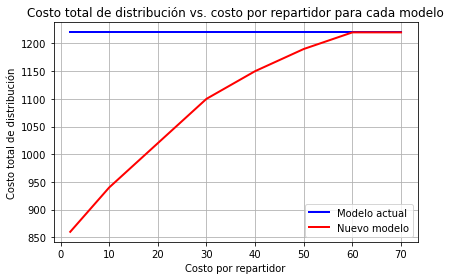
\includegraphics[width=0.6\textwidth]{costo_tot_vs_costo_rep.png}
        \caption{Costo total vs. costo por repartidor para cada modelo}
        \label{fig:mi-imagen}
    \end{figure}


    \begin{figure}[H]
        \centering
        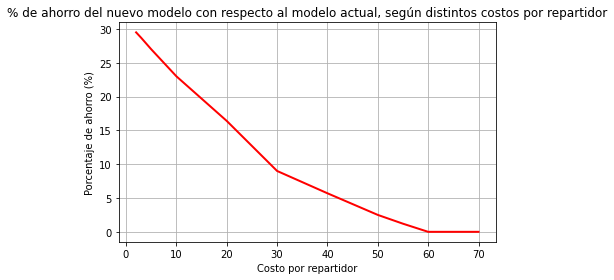
\includegraphics[width=0.8\textwidth]{porcentaje_ahorro_vs_costo_rep.png}
        \caption{Porcentaje de ahorro en costo total de distribución para el Nuevo Modelo en comparación con el Modelo Actual, según distintos costos por repartidor}
        \label{fig:mi-imagen}
    \end{figure}

    De estos resultados, podemos observar que si la empresa implementara el Nuevo Modelo y pagara \$30 o menos por cada reparto realizado por repartidor, la rentabilidad de la empresa mejoraría significativamente, pues generaría un ahorro en costos de distribución mayor al 9,0\%. De hecho, si la empresa lograra conseguir repartidores que cobren \$5 por viaje o menos, se reducirían los costos de entrega en un 27\% que es un ahorro muy significativo. \\
    También observamos que si no se lograsen conseguir repartidores que cobren menos de \$55 por viaje, entonces definitivamente no valdría la pena implementar el Nuevo Modelo, pues el ahorro sería prácticamente nulo. \\
    Concluimos que, ante estas condiciones de este experimento, si la empresa pudiera pagar a sus repartidores una suma de \$30 o menos por reparto, entonces sí le sería muy beneficiosa la aplicación del Nuevo Modelo.


    \subsubsection{Experimento 2: variación de densidad de clientes en la ciudad}

    Todos los parámetros de este experimento se mantienen iguales que en el experimento anterior (20 clientes ubicados al azar, distancia máxima de recorrido de repartidores 5 km, un 25\% de los clientes fueron elegidos al azar para que sean quienes requieren productos refrigerados y el costo de cada tramo hecho por camión es igual a 10 veces la distancia de ese tramo), solo que ahora quedó fijo el costo por reparto de repartidor en \$10 y lo que se variará será la densidad de clientes de la ciudad (número de clientes por $km^{2}$). En el caso "ciudad muy densa" se acomodarán los 20 clientes en un área de  $100$ $km^{2}$; en el caso "ciudad densa" en un área de $400$ $km^{2}$; para "ciudad moderada" un área de $1600$ $km^{2}$; para "ciudad dispersa" un área de $6400$ $km^{2}$; y para el caso de "ciudad muy dispersa" un área de $25600$ $km^{2}$.  \\
    Lo que se busca en este experimento, es ver qué tan beneficiosa sería la aplicación del Nuevo Modelo con respecto al modelo tradicional, en contextos de ciudades de distintas densidades de clientes por $km^{2}$. \\
    \\
    He aquí los resultados:

    \begin{table}[H]
    \centering
    \resizebox{\textwidth}{!}{
    \begin{tabular}{|c|c|c|c|c|}
    \hline
    \textbf{Densidad ciudad} & \textbf{Costo Modelo Actual} & \textbf{Costo Nuevo Modelo} & \textbf{Repartidores requeridos} & \textbf{Ahorro (\%)} \\
    \hline
    Muy densa & 350 & 200 & 16 & 42,9\% \\
    Densa & 820 & 640 & 11 & 22,0\% \\
    Moderada & 1440 & 1350 & 4 & 6,3\% \\
    Dispersa & 3180 & 3010 & 3 & 5,4\% \\
    Muy dispersa & 6450 & 6450 & 0 & 0\% \\
    \hline
    \end{tabular}
    }
    \caption{Comparación de costos entre metodologías para distintas densidades de clientes por $km^{2}$}
    \end{table}

    Como era de esperar, observamos que el uso de repartidores a pie/bicicleta resulta muy beneficioso en ciudades de alta densidad poblacional. Al ser la densidad de clientes alta, estos distan poco entre ellos. Muchas de esas distancias son menores a la distancia máxima permitida para los repartidores, por lo que muchas de las entregas podrán ser realizadas por estos, lo cual abarata muchísimo los costos de distribución de mercadería. De hecho se observa en el caso de la ciudad densa, que el 80\% de los repartos se hizo a través de repartidores. El camión debió usarse solo para llegar a 4 clientes. \\
    A medida que la densidad poblacional se achica, se agrandan las distancias entre clientes y naturalmente se agrandan los costos de distribución total tanto para el Modelo Actual como para el Nuevo Modelo. Pero observando la columna "Ahorro" observamos que, a menor densidad poblacional, menos beneficio obtenemos de implementar el Nuevo Modelo. Esto tiene mucho sentido: a menor densidad poblacional, más grandes las distancias cliente-cliente y menos viajes factibles para hacer por repartidores, entonces es cada vez menor la diferencia que implicaría el aplicar el modelo nuevo con respecto al actual. De hecho, vemos el caso extremo en la ciudad muy dispersa, donde ningún viaje puede/conviene hacerse por repartidor, entonces el modelo nuevo no produce ninguna mejora en la rentabilidad con respecto al modelo anterior. \\
    Concluimos que la aplicación del Nuevo Modelo puede ser útil o no, de acuerdo a la densidad de clientes que posea la ciudad. Y es especialmente útil en ciudades muy densas, donde el servicio de los repartidores será altamente utilizado.


    \subsection{Evaluación de pérdida al considerar restricciones deseables}
    Realizaremos experimentos sobre los nuevos modelos con las restricciones adicionales tanto por separado como con la combinación de ambas.\\
    Nuestro objetivo es verificar como la restricciones deseadas por el cliente afectan al valor de la solución óptima.


    \subsubsection{Experimento 3: variación de número de clientes exclusivos}

    En este experimento comparamos el Nuevo Modelo con el Modelo Adicional con clientes requeridos. Trabajamos con una ciudad de tamaño $900$ $km^{2}$, con 20 clientes totales. Al igual que en el experimento anterior el costo por repartidor se fijó en 10, la máxima distancia recorrible por repartidores en 5 km, la cantidad de clientes que requieren productos refrigerados también corresponde a un 25\% de los clientes, elegidos al azar, y el costo por cada tramo hecho por un camión equivale a 10 veces la longitud de ese tramo. Lo que se irá variando en este experimento, es la cantidad de "clientes exclusivos" (clientes que deben recibir la mercadería sí o sí entregada por el camión). \\
    \\
    Aquí se presentan los resultados:

    \begin{table}[H]
    \centering
    \resizebox{\textwidth}{!}{
    \begin{tabular}{|c|c|c|c|c|c|c|}
    \hline
    \thead{Nro. exclusivos} & \thead{Costo \\ Nuevo Modelo} & \thead{Costo Modelo \\ Adicional de exclusivos} & \thead{Costo Modelo \\ Adicional Combinado} & \thead{Envios realizados \\ por repartidores} & \thead{Pérdida Modelo \\ Adicional (\%)} & \thead{Pérdida Modelo \\ Adicional Combinado (\%)}\\
    \hline
    1  & 920   & 920  & 980  & 7  | 7 | 8 & 0\%     & 6,5\%\\
    2  & 1100  & 1110 & 1230 & 5  | 5 | 0 & 0,9\%  & 11,8\%\\
    5  & 950   & 980  & 1110 & 6  | 4 | 0 & 3.1\%  & 16,8\%\\
    10 & 1010  & 1150 & 1150 & 8  | 3 | 0 & 8,9\%  & 13,9\%\\
    15 & 1010  & 1140 & 1160 & 8  | 2 | 4 & 12,8\% & 14,9\%\\
    20 & 790   & 980  & 980  & 10 | 0 | 0 & 24,9\% & 24,9\%\\
    \hline
    \end{tabular}
    }
    \caption{Comparación de costos entre Nuevo Modelo y Modelo Adicional para diferentes cantidades de clientes exclusivos}
    \end{table}
    Se puede apreciar como al agregar la restricción de que un conjunto de clientes deba ser visitado por el camión se puede llegar a casos donde aumente el costo del reocorrido.
    Sin embargo, no se observa un patrón claro de perdida dependiendo de la cantidad de clientes exclusivos de cada instancia.\\
    Parecería que el porcentaje de pérdida que tenemos al aplicar el Modelo Adicional es muy sensible a la disposición de la ciudad (o sea, a las distancias cliente-cliente), entonces no podemos sacar conclusiones claras acerca de la relación entre la aplicación de este modelo con respecto al número de clientes exclusivos. \\
    Lo único que sí parece claro es que al aumentar el número de clientes exclusivos, más probable parece ser que el número de pedidos realizados por repartidores sea 0, lo cual tiene sentido. \\
    Para hacer un buen análisis del impacto de de la aplicación del Modelo Adicional, lo ideal sería trabajar con una instancia (ciudad) específica.

    \subsubsection{Experimento 4: Modelo Adicional ante ciudades con distintas densidades de clientes}

    En este experimento trabajamos con las mismas instancias "ciudad densa", "ciudad dispersa", "ciudad muy densa", "ciudad moderada" y "ciudad muy dispersa" del experimento 2. Pero ahora, sobre cada una de ellas probaremos el Nuevo Modelo y el Modelo Adicional con restricciones sobre los repartidores.

    \begin{table}[H]
    \centering
    \resizebox{\textwidth}{!}{
    \begin{tabular}{|c|c|c|c|c|}
    \hline
    \textbf{Densidad ciudad} & \textbf{Costo Nuevo Modelo} & \textbf{Costo Modelo Adicional (repartidores)} & \thead{Envios realizados \\ por repartidores} & \textbf{Pérdida (\%)} \\
    \hline
    Muy densa    & 200  & 200  &  16 | 16 & 0\% \\
    Densa        & 640  & 780  &  8 | 11 & 22,0\% \\
    Moderada     & 1350 & 1440 &  0 | 4   & 6,7\% \\
    Dispersa     & 3010 & 3180 &  0 | 3   & 5,6\% \\
    Muy dispersa & 6450 & 6450 &  0 | 0   & 0\% \\
    \hline
    \end{tabular}
    }
    \caption{Comparación de costos entre metodologías para distintas densidades de clientes por $km^{2}$}
    \end{table}

    Observamos que en general cuanto más densa es la ciudad en clientes, más diferencia habrá entre el costo total de distribución para Nuevo Modelo y Modelo Adicional. Esto es así pues, como vimos antes, para ciudades densas se favorece mucho la utilización de repartidores. En Nuevo Modelo se aprovechan al máximo los repartidores, si el modelo lo requiere, ellos están disponibles. En cambio en Modelo Adicional, se necesitan más requisitos para que se contraten repartidores. De esta forma se pueden desaprovechar grandes oportunidades de ahorro. \\
    Por el contrario, cuanto más dispersa es la ciudad en clientes, más distancia cliente-cliente, menos repartidores podrán ser usados en ambos modelos y por ende, no se generará tanta diferencia entre modelo y modelo. \\
    También notamos que si la ciudad ya pasa a ser muy densa, baja la pérdida, y esto puede deberse a que al ser tan densa la restricción de que salgan 4 repartidores por punto deja de ser un problema porque hay muchos puntos a los que se puede llegar en bicicleta desde cada cliente del camión, y podrían seguir usándose tantos repartidores como antes.

    Al correr el modelo de restricciones adicionales combinadas obtuvimos los mismos resultados, salvo para la ciudad muy densa donde se obtuvo una pérdida del 20,0\%: el exigir que ciertos clientes tengan que recibir sí o sí su pedido por camión, hace que el recurso de los repartidores que tan bien le viene a las ciudades muy densas en clientes, no se pueda explotar. La pérdida es bastante significativa.

    \subsection{Análisis del tiempo de cómputo para distintos parámetros de CPLEX}

    Al realizar los experimentos, lo primero que resalta es la diferencia en tiempos de ejecución de los distintos modelos. TSP suele darnos resultados bastante rápido (segundos) para entradas en las cuales el modelo con repartidores tarda bastante (10 minutos o más incluso). También notamos que las mismas instancias pero corriendo el modelo con las restricciones adicionales tardaba inclusive más. Por ejemplo para el modelo con las dos restricciones adicionales juntas, había casos en que tsp tardaba menos de 10 segundos, el modelo con repartidores alrededor de 15 minutos, pero el modelo con ambas restricciones más de una hora.

    Teniendo esto en cuenta, tomamos solo el modelo de repartidores para analizar si cambiando algún parámetro del algoritmo de CPLEX podíamos mejorar los tiempos de cómputo. Nos concentramos solo en este modelo y no en el de las restricciones adicionales para no extendernos tanto.


    \subsubsection{Experimento 5: variación en los parámetros de CPLEX}
    La idea de esta sección es encontrar si algún cambio en las decisiones del algoritmo de CPlex podía disminuir en general el tiempo de cómputo. Para empezar, hicimos una búsqueda intensa para un caso particular para tener un primer pantallazo de qué parámetros podían implicar una mejora en el tiempo.

    Tomamos una instancia con 55 nodos, costo de repartidor 7, 5 envíos refrigerados, y distancia de repartidor 100. Y los resultados fueron los siguientes:

    \begin{table}[H]
    \centering
    \resizebox{0.5\textwidth}{!}{
    \begin{tabular}{|c|c|}
    \hline
    \textbf{Parámetros cambiados} & \textbf{Tiempo (segundos)} \\
    \hline
    Default & 866 \\
    \hline
    Node Select: DFS & 633 \\
    Node Select: Best Estimated & 858 \\
    Node Select: Best Estimated Alternative & 4872 \\
    \hline
    Variable Select: Strong Branching & 2119 \\
    Variable Select: Pseudo Costs & 7950 \\
    Variable Select: Min Infeasibility & $>$24817 (aborted*) \\
    Variable Select: Max Infeasibility & $>$6383 (aborted*) \\
    \hline
    Heurística Primal: Increase = 2 & 927 \\
    Heurística Primal: None & 1348 \\
    Heurística Primal: Decrease = 0.5 & 7734 \\
    \hline
    Cortes raíz: None & $>$3721 (aborted*)\\
    Cortes raíz: Aggresive & 854\\
    \hline
    Cortes árbol: None & 1632\\
    Cortes árbol: Aggresive & $>$2240 (aborted*)\\
    \hline
    Cortes Gomory: None & 1620\\
    Cortes Gomory: Aggresive & $>$1641 (aborted*)\\
    \hline
    Node DFS + Cortes raíz aggresive & 575 \\
    Node Best estimated + Cortes raíz aggresive & 1077 \\
    \hline
    \end{tabular}
    }
    \caption{Comparación de tiempos según los parámetros de CPLEX}
    \end{table}

    \textit{(*) Las instancias abortadas se deben a que consumían mucho tiempo, y notábamos que aún le faltaba bastante para converger (tenían pocos cierres de nodos, y avanzaban muy lento en cada nodo, o muchas iteraciones que no tenían mejoras). Y como de todas maneras el tiempo que requerían ya era significativamente mayor al original, las cortamos para poder probar con otras decisiones.}
    \vspace{3mm}

    A partir de este caso disparador, tomamos la selección de nodos con DFS, y DFS + cortes agresivos en el nodo raíz, y nos interesa ver si realmente en general mejoran el tiempo de ejecución en nuestro modelo de TSP+repartidores.

    Mientras corríamos los experimentos buscando algunos que tarden un tiempo razonable para analizar, una cosa que notamos es que hay tres cosas que en particular aumentan el tiempo de cómputo:
    \begin{itemize}
        \item La cantidad de nodos:
        \begin{itemize}
            \item A mayor cantidad de nodos mayor el tiempo.
        \end{itemize}

        \item La distancia máxima del repartidor respecto a las distancias entre ciudades:
        \begin{itemize}
            \item Para una misma ciudad, si aumentamos la distancia máxima del repartidos (hay más opciones a las que puede llegar en bici), más tarda en ejecutar.
        \end{itemize}

        \item El costo del repartidor respecto a los costos del camión:
        \begin{itemize}
            \item Para una ciudad dada y manteniendo fijos los costos del camión, si aumentamos el costo del repartidor, acercándolo a los del camión  (es decir, los costos son más competitivos), más tarda en ejecutar.
        \end{itemize}
    \end{itemize}

    Entonces empezamos a generar distintas instancias, jugando con la cantidad de nodos, el costo del repartidor y la distancia máxima del mismo. Dejamos que los costos y distancias entre ciudades se generen de manera aleatoria (fijando el máximo para cada uno). (No variamos la cantidad de clientes con productos refrigerados, tampoco).

    Así, llegamos a los siguientes resultados:

        \begin{table}[H]
    \centering
    \resizebox{0.9\textwidth}{!}{
    \begin{tabular}{|c|c|c|c|c|c|c|c|}
    \hline
    \textbf{Cantidad} & \textbf{Costo} & \textbf{dist max} & \textbf{Tiempo} & \textbf{tiempo} &  \textbf{tiempo dfs +} & \textbf{\% tiempo} & \textbf{\% tiempo dfs + } \\
    \textbf{nodos} & \textbf{repartidor} &   & \textbf{default} & \textbf{dfs} & \textbf{raiz aggresive cut} & \textbf{dfs} & \textbf{raiz aggresive cut}\\
    \hline
    40 & 12 & 80 & 121 & 95 & 167 & 78.51\% & 138.02\% \\
    40 & 12 & 100 & 312 & 244 & 293 & 78.21\% & 93.91\% \\
    45 & 24 & 80 & 913 & 803 & 712 & 87.95\% & 77.98\% \\
    50 & 12 & 80 & 2544 & 1518 & 1891 & 59.67\% & 74.33\% \\
    55 & 30 & 80 & 698 & 474 & 1360 & 67.91\% & 194.84\% \\
    55 & 20 & 15 & 1002 & 788 & 1269 & 78.64\% & 126.65\% \\
    60 & 8 & 100 & 2053 & 1482 & 1789 & 72.19\% & 87.14\% \\
    60 & 8 & 80 & 888 & 587 & 1433 & 66.10\% & 161.37\% \\
    60 & 27 & 80 & 6989 & 6761 & 3250 & 96.74\% & 46.50\% \\
    \hline
    \end{tabular}
    }
    \caption{Comparación de tiempos para varias instancias}
    \end{table}

    Notamos que el tiempo de ejecución con selección de nodos por dfs en todos los casos implicó un ahorro de tiempo, a lo sumo varía que tanto impacto. Esto nos parecería indicar que para una instancia cualquiera de nuestro problema, usar dfs va a ser más rápido que la configuración totalmente defalut. 
    
    En cambio el ahorro de tiempo de combinar la selección con dfs, y usar planos de cortes agresivos en el nodo raíz, depende mucho de la instancia. EN algunas significó un ahorro incluso mayor que con dfs, en otras se mantuvo similar, y en otras empeoró bastante. No notamos ningún patrón claro que indique cuando puede mejorar y cuánto empeorar. Pero esto nos marca que cada instancia particular puede tener una combinación de parámetros óptima particular a sí misma.

    \section{Conclusiones}
    \subsection{Ganancia de implementar la nueva metodología}
    Según los resultados obtenidos, notamos que el costo del repartidor y la densidad de la ciudad (o la distancia máxima del repartidor) son significativos en cuanto a la ganancia obtenida.

    Si el costo del repartidor es barato, por lo general va a ser conveniente el método que agrega el uso de repartidores.

    Sin embargo también hay que tener en cuanta la densidad de la ciudad / la distancia máxima del repartidor. Mientras más ciudades se pueda llegar en bicicleta desde un punto, más va a ser el ahorro. Lo cuál es lógico porque puedo hacer un recorrido corto en camión, y desde cada punto cubrir el resto con repartidores.

    Por lo tanto, si se tiene un equilibrio en la distancia que puede cubrir un repartidor, y el costo del mismo, el ahorro puede ser muy significativo. Pero mientras más restrinja a los repartidores, o más caros sean, podría llegar incluso o no presentar ningún beneficio.

    \subsection{Pérdida de implementar restricciones adicionales}
    En caso de tanto la restricción a los repartidores como al implementar ambas restricciones, notamos que la pérdida afectará particularmente a las ciudades densas. Esto tiene sentido si pensamos que estas eran las que más ahorro tenían al poder usar repartidores. Pero al poner clientes exclusivos, y pedir que no haya menos de cuatro pedidos por repartidor desde cada punto, reducimos la libertad para explotar ese beneficio. Por lo tanto, gran parte del ahorro que habíamos tenido se podría ver afectado.

    En cambio en el caso de ciudades más dispersas, ya de por sí el ahorro era poco, al usar pocos repartidores, por lo tanto, incluir estas restricciones no empeorará mucho, ya que como mucho va a ser tan costoso como TSP.
    
    En cuanto a la otra restricción, la cantidad de clientes exclusivos también puede afectar la ganancia, sin embargo la pérdida en este caso no es tan lineal. Esto puede deberse a que va a depender de qué nodos son marcados para ser exclusivos. Si justo elegimos varios que de todas formas convenía que pase el camino del camión, no se verá afectado.

    Será conveniente tener cuidado entonces con el caso particular del cuál partimos, y de la cantidad de ciudades exclusivas marcadas, qué tanta pérdida respecto a la ganancia original representa agregar estas restricciones.

    \subsection{Tiempo de cómputo}
    Notamos que el tiempo de cómputo depende fuertemente no solo del tamaño de la instancia (cantidad de clientes), sino de todos sus parámetros. En particular, notamos un fuerte aumento en el tiempo de cómputo al tener costos de repartidor cada vez más cercanos a los del camión, y distancia del repartidor cada vez más abarcativa respecto a las distancias de los clientes.
    
    Ahora, en cuanto a optimizar el algoritmo, las pruebas nos permiten concluir que es conveniente en general (para todos los casos en los que probamos) usar la selección de nodos con dfs. 
    
    Sin embargo, cada caso en particular puede tener alguna combinación mejor de parámetros. Esto se ve en el primer intento, donde la combinación de usar selección de nodos con dfs y planos de cortes agresivos en el nodo raíz nos daba el mejor tiempo, pero al usar esa combinación en otros problemas ya no se mantuvo la propiedad como con dfs. 
    
    Por lo tanto, sería conveniente para el caso general usar la combinación de parámetros default cambiando la selección de nodos por dfs.
    
    \end{document}